\chapter{Results}
\label{results}

In this chapter, we present the results of anomaly detection experiments performed with two different feature embeddings. We use two methods of evaluation: comparing the metrics of accuracy, precision, recall and $F1$ to evaluate the performance with the labeled test dataset and validating the results using domain experts.

Numerical validation of the models will give us a conclusive answer to \textbf{RQ1}. To answer \textbf{RQ2}, we will compare the validation metrics computed for both the event count and TF-IDF representations. Finally, we use the test set to evaluate the performance of the selected anomaly detection algorithms in answering \textbf{RQ3}. A thorough analysis of these results along with the help of expert validation at the end of this chapter will directly address \textbf{RQ4}.

Proper evaluation is a crucial step in machine learning. Supervised methods typically check how the model performs on the training data, as well as on previously unseen datasets called \textit{test} or \textit{validation}, using various performance metrics. If the results are not satisfactory, this information can be used to optimize the model's hyperparameters and repeat the process. However, in the case of unsupervised learning, which we used in our research, it is not immediately obvious how to approach model evaluation. 

The only dataset we can consider labeled is the Nightly dataset used for training. All the data collected during the night are \textit{normal} instances without anomalies, but we need to test whether the actual anomalies are detected by our detectors and whether the detected anomalies match actual anomalies. 

As described in Chapter \ref{chapter:dataset} when defining our datasets, we manually created a test set of logs containing two types of observed anomaly scenarios that are included in the Anomalies dataset: Killing the Redis server and Killing the RabbitMQ message broker. In our simulations of these scenarios, we know the specific time range in which an anomaly occurs, so we can hand-label certain feature embeddings. Also, a portion of the Nightly Test dataset that contains data not seen during the training phase is used as part of the test dataset. Finally, we include the Glostrup Calling dataset in our test set, which contains a set of log messages generated during calls, as it is very important that our models do not detect calls as anomalies.

The weakness of this approach is that there are only two known types of anomalies in the test dataset. There is no way to tell if the models behave correctly on live and production data. As a compromise, we use the Daily dataset whose labels are unknown to generate predictions. We then perform what we call \textit{expert validation}. We ask domain experts from the Motorola Solutions SmartConnect team to evaluate a small subset of the predictions generated by our best-performing models. 


\section{Test Dataset Validation}

The interpretation of the anomaly detection models by the evaluation metrics obtained on the test set (Section \ref{section:testset}) containing two types of anomalies helped us to verify the \textbf{RQ1} proposed in Chapter \ref{introduction}, that the logs generated by Motorola SmartConnect are indeed generated in such a way that they can be used for anomaly detection. Let us now take a closer look at the results of the machine learning algorithms that allow us to answer the remaining research questions.

Table \ref{tab:results} shows the summarized experiment results on the test dataset for the models Isolation Forest, PCA, Invariants Mining and Log Clustering. We first compare the results in terms of feature embeddings and then discuss how the different anomaly detection algorithms performed in comparison to each other.  

\begin{table}[h]
\centering
\resizebox{\textwidth}{!}{\begin{tabular}{@{}cccccc@{}}
\toprule
\textbf{Algorithm}         & \textbf{Embedding}                                           & \textbf{Precision}                                         & \textbf{Recall}                                             & \textbf{F1}                                                 & \textbf{Accuracy}                                           \\ \midrule
\textcolor{customGreen}{\textbf{Isolation Forest}}  & \begin{tabular}[c]{@{}c@{}}Event count\\ TF-IDF\end{tabular} & \begin{tabular}[c]{@{}c@{}}100.00\%\\ 33.33\%\end{tabular}  & \begin{tabular}[c]{@{}c@{}}57.14\%\\ 14.81\%\end{tabular}   & \begin{tabular}[c]{@{}c@{}}66.67\%\\ 20.51\%\end{tabular}    & \begin{tabular}[c]{@{}c@{}}87.79\%\\ 76.15\%\end{tabular}    \\ \midrule
\textcolor{customGreen}{\textbf{PCA}}               & \begin{tabular}[c]{@{}c@{}}Event count \\ TF-IDF\end{tabular} & \begin{tabular}[c]{@{}c@{}}100.00\%\\ 100.00\%\end{tabular} & \begin{tabular}[c]{@{}c@{}}100.00\%\\ 100.00\%\end{tabular} & \begin{tabular}[c]{@{}c@{}}100.00\%\\ 100.00\%\end{tabular}  & \begin{tabular}[c]{@{}c@{}}100.00\%\\ 100.00\%\end{tabular}  \\ \midrule
\textcolor{customGreen}{\textbf{Invariants Mining}} & \begin{tabular}[c]{@{}c@{}}Event count\\ TF-IDF\end{tabular} & \begin{tabular}[c]{@{}c@{}}22.22\%\\ 21.60\%\end{tabular}   & \begin{tabular}[c]{@{}c@{}}100.00\%\\ 100.00\%\end{tabular}  & \begin{tabular}[c]{@{}c@{}}36.36\%\\ 35.53\%\end{tabular}    & \begin{tabular}[c]{@{}c@{}}25.19\%\\ 24.62\%\end{tabular}    \\ \midrule
\textcolor{customGreen}{\textbf{Log Clustering}}    & \begin{tabular}[c]{@{}c@{}}Event count\\ TF-IDF\end{tabular} & \begin{tabular}[c]{@{}c@{}} 100.00\%\\  100.00\%\end{tabular}          & \begin{tabular}[c]{@{}c@{}}100.00\%\\ 100.00\%\end{tabular} & \begin{tabular}[c]{@{}c@{}}100.00\%\\ 100.00\%\end{tabular} & \begin{tabular}[c]{@{}c@{}}100.00\%\\ 100.00\%\end{tabular} \\ \bottomrule
\end{tabular}}
 \caption{The precision, recall, F1 score, and accuracy for anomaly detection methods computed on the test dataset with two different embeddings: Event Count and TF-IDF. Both embeddings are generated with a sliding window of two minutes.}
    \label{tab:results}
\end{table}


\subsection{Feature Embeddings Comparison}
To address \textbf{RQ2}, we wanted to see how different feature embeddings in a numeric vector affected the results. As described in previous chapters, we proposed two embeddings: a simple event count vector and a weighted TF-IDF vector. TF-IDF is obtained from event count weight by giving more weight to events that occur less frequently in the whole dataset. We wanted to see if this type of information could bring more knowledge that would be beneficial to the anomaly detection model.

From the results, both embeddings perform very similarly, and it is not possible to tell from the test dataset which one would perform better on unknown anomalies. If we compare in Figure \ref{fig:tf-vs-tfidf} the t-SNE visualization applied to normal data points and anomaly data points of different embeddings, we can see that both event count and TF-IDF treat anomalies and normal data in a similar way. Both event count embedding and TF-IDF embedding produced clusters in the embedding space that are visually visible and can distinguish between normal and anomalous data points.

Another means of comparing these two embeddings is by looking at the histogram in Figure \ref{fig:histogram-event-types}. We expected TF-IDF to assign a higher value to events that occur infrequently, which we hypothesized should include events that are representative of anomalies. The histograms seem to agree in the middle part of the plot, but for the first five hundred event type IDs a much lower weight is observed in the TF-IDF histogram compared to the event count histogram. After manually inspecting the feature vectors, we noticed a pattern in the frequency of event types with lower IDs. The corresponding event types occur with identical frequency in successive log sequences. This is to be expected and makes sense since the events behind these event type IDs include starting a call, attempting to start a new TLS connection, and other regularly occurring events. Therefore, these event types can be considered as frequently occurring events, which is why the TF-IDF algorithm assigns them a lower weight, which is reflected in the histogram.

All in all, considering that event count embedding is simple and much easier to interpret than TF-IDF and TF-IDF did not perform significantly better in the test dataset, we consider event count embedding as the preferred representation of the dataset for practical use.


% Distribution graph to compare the TF IDF to see how many TFIDF had high occurency


\begin{figure}[h]%
    \centering
    \subfloat[\centering Event count embedding]{{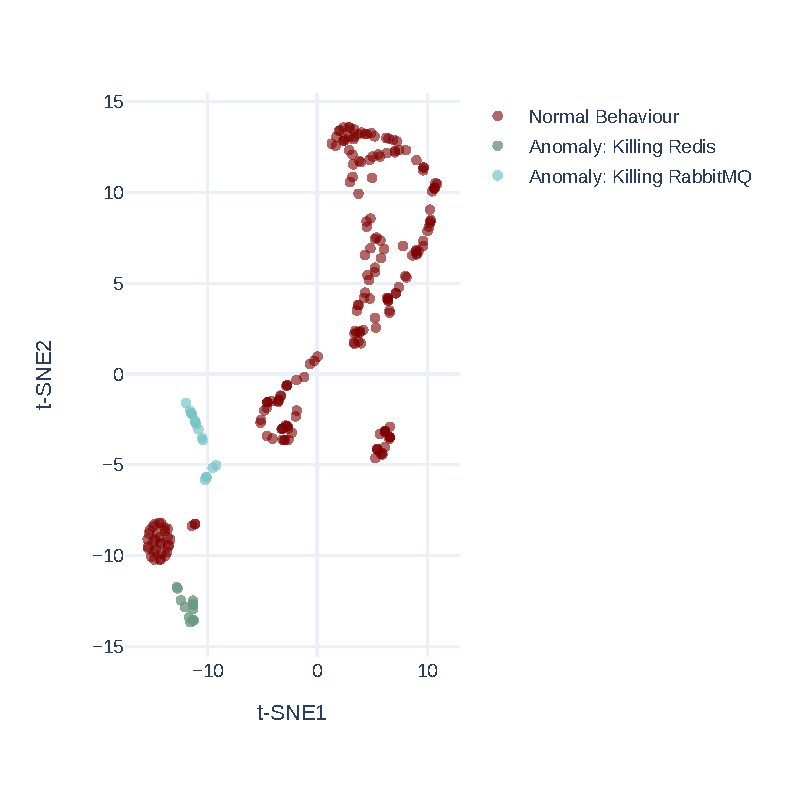
\includegraphics[width=5.52cm]{img/tsne-anomalies-vs-normal-small.pdf}}}%
    \qquad
    \subfloat[\centering TF-IDF embedding]{{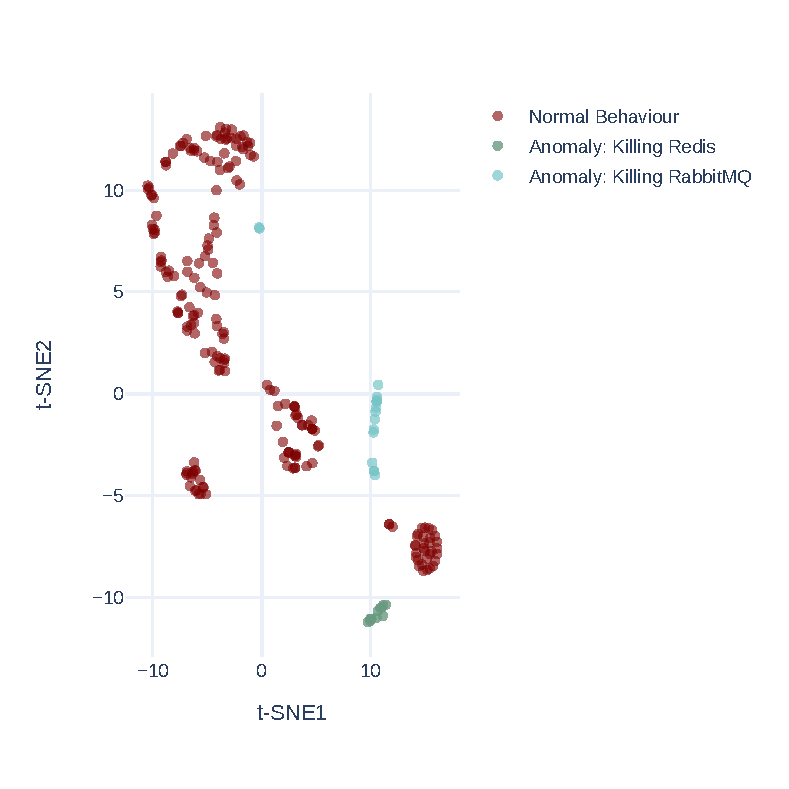
\includegraphics[width=5.52cm]{img/tsne-anomalies-vs-normal-tfidf.pdf}}}%
    \caption{Event count embedding (left) and TF-IDF embedding (right) of the normal and anomalous log sequences plotted using PCA.}%
    \label{fig:tf-vs-tfidf}%
\end{figure}

\begin{figure}[h]%
    \centering
    \subfloat[\centering Event count]{{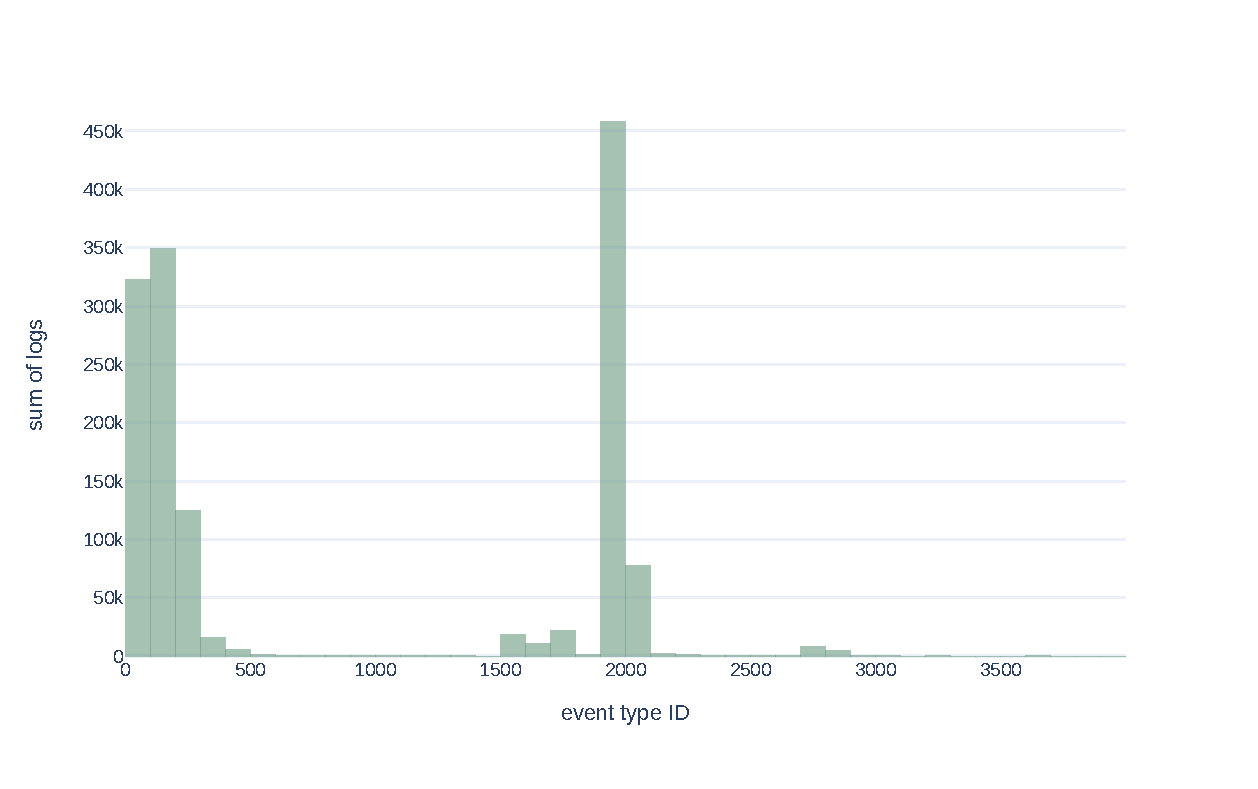
\includegraphics[width=0.9\textwidth]{img/tf-histogram.pdf}}}%
    \qquad
    \subfloat[\centering TF-IDF]{{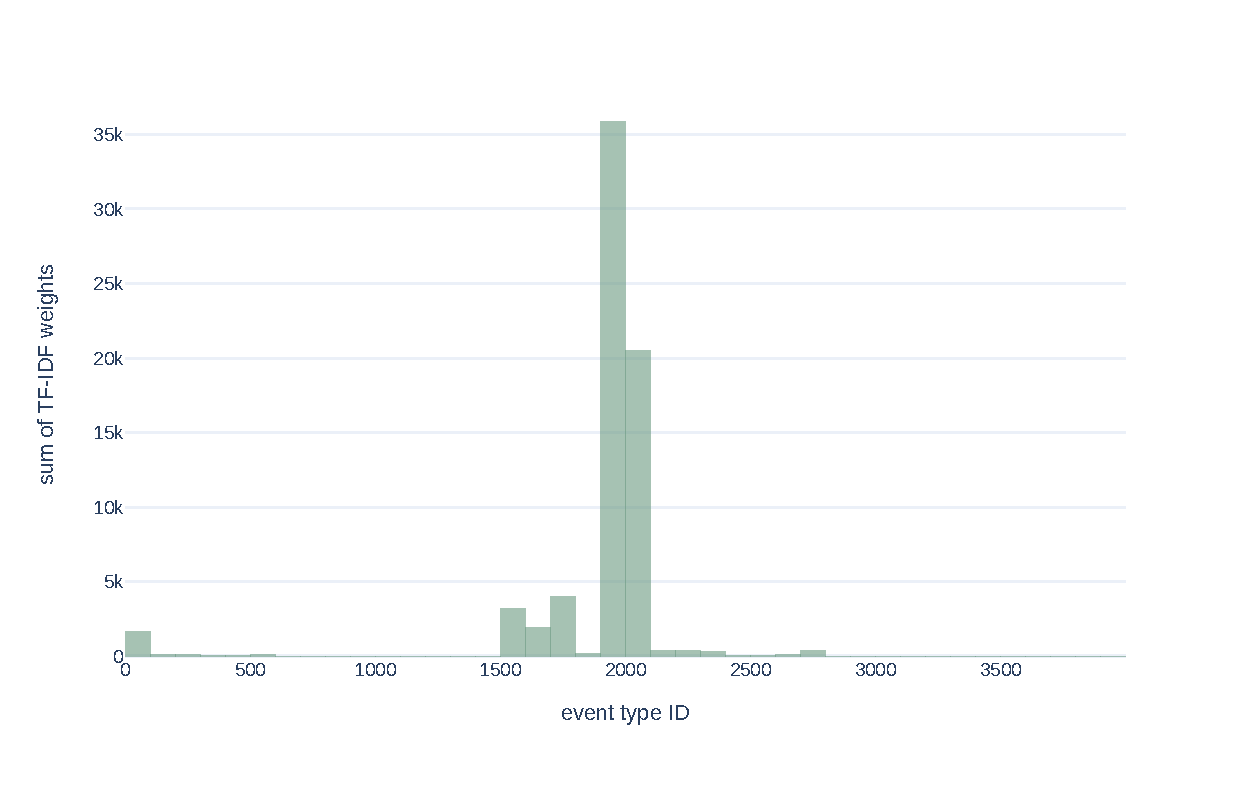
\includegraphics[width=0.9\textwidth]{img/tfidf-histogram.pdf}}}%
    \caption{Histogram distribution plot of the event type IDs in the test dataset, where the logs of the same event type ID, shown on the x-axis, are binned together and their cumulative count is shown on the y-axis. (a) is a histogram generated over event count embeddings, and (b) is a histogram generated over TF-IDF embeddings.}%
    \label{fig:histogram-event-types}%
\end{figure}


\subsection{Anomaly Detection Methods Comparison}
In this section, we describe how well do the four proposed anomaly detection methods perform on the labeled test dataset. To support our reasoning, we refer to the reported experimental results using evaluation metrics for embedding the test dataset with a two minute sliding window from Table \ref{tab:results}. 

In order of importance, it is more important for a live production system not to miss an anomaly than to correctly detect anomaly-free data points. In other words, false negatives are more alarming than false positives. To analyze the ratio of identified anomalous and non-anomalous log sequences within all datasets, we derived confusion matrices for the Isolation Forest, PCA, Invariants Mining and Log Clustering models, which are shown in Table \ref{table:confusionMatrix:if}, Table \ref{table:confusionMatrix:pca}, Table \ref{table:confusionMatrix:im} and Table \ref{table:confusionMatrix:clustering}. Figure \ref{fig:tsne-predictions-labeled} gives a visual interpretation of which points were misclassified in each anomaly detection method. 

From the results table, it can be seen that all the anomaly detection methods give a decent result, with Log Clustering and PCA performing significantly better than Invariants Mining and Isolation Forest.  

Among the four unsupervised anomaly detection algorithms, the evaluation metrics for Invariants Mining model are the lowest with the values of $22.22\%$ precision, $100.00\%$ recall and $36.36\%$ F1 score. Figure \ref{fig:tsne-predictions-labeled} (c) shows that Invariants Mining has a tendency to falsely identify normal data points as anomalies. This poor performance is not surprising and we suspect that there are two reasons for this occurrence. First, as explained in Section \ref{section:experimental-setup}, we did not perform hyperparameter exploration because the training process for Invariants Mining on our dataset is extremely ineffective. However, we assume that the main reason for the inability to detect anomalies is the way we performed windowing in log sequences. In similar research that successfully used Invariants Mining, such as He et al. \cite{he2016}, they used \textit{session ID} or \textit{process ID} shared between logs as a key for grouping logs into log sequences. We, on the other hand, focused on the timely relationship between logs and grouped them into log sequences in consecutive two-minute windows. Therefore, there is no guarantee that log events that are part of the invariants revealed by Invariants Mining are in the same log sequence in the resulting embedding. Therefore, it is expected that the Invariants Mining method does not perform well in the feature representation of our log dataset.

Another algorithm that did not perform well is Isolation Forest with $100\%$ precision, but $57.14\%$ recall and $66.67\%$ F1 score. In \ref{fig:tsne-predictions-labeled} (a), we can observe that Isolation Forest misses a high number of anomalies, resulting in low recall and a high number of false negatives as well as false positives. We concluded that one reason for this finding is that Isolation Forest is not well suited for the one-class learning case (training set containing only negative samples) \cite{adForest}. The leaves of iTrees provide an anomaly score equal to the length of the average path from the node (sample from the training set) to that leaf. The shorter the path, the smaller the anomaly score and the higher the probability that it is an outlier. Since all samples in the training dataset are normal, assigned anomaly scores may be biased. Therefore, the performance of Isolation Forest does not perform well on our dataset.

Log clustering and PCA achieved superior performance compared to other anomaly detection methods proposed in our research. The final result is $100.00\%$ precision, recall, F1 score and accuracy on the test dataset for both Log Clustering and PCA. It is of our interest to investigate these two algorithms further, and in the next section we will ask the developers of Motorola Solutions to evaluate the results of these two algorithms on a previously unseen dataset (Daily) for which we have no labels and only experts knowledgeable in the field can say whether the predictions are correct.  

\begin{figure}%
    \centering
    \subfloat[\centering Isolation Forest]{{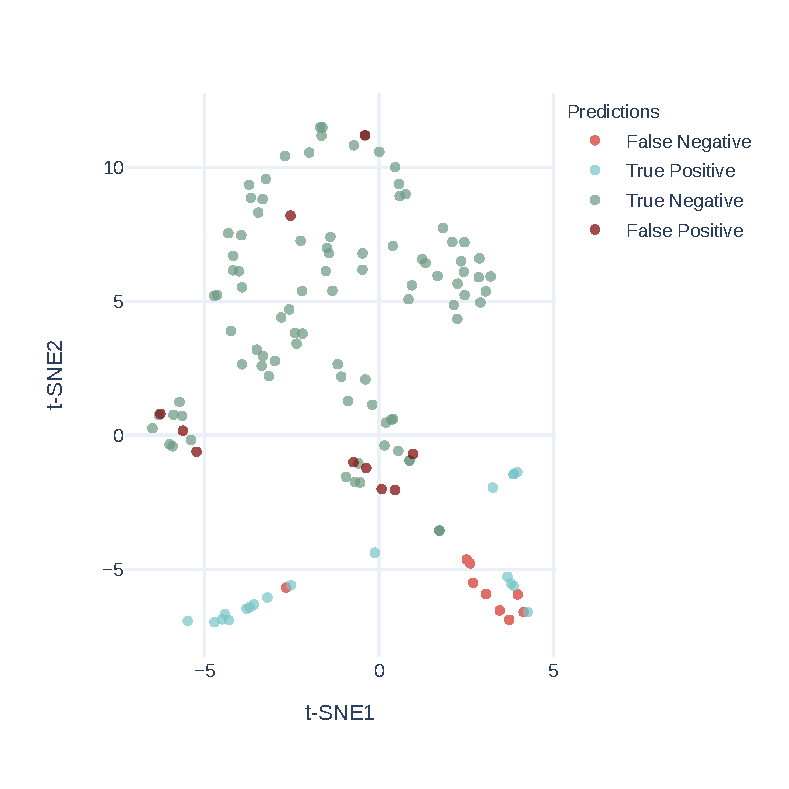
\includegraphics[width=5.52cm]{img/tsne-predictions-isolation-forest.pdf}}}%
    \qquad
    \subfloat[\centering PCA]{{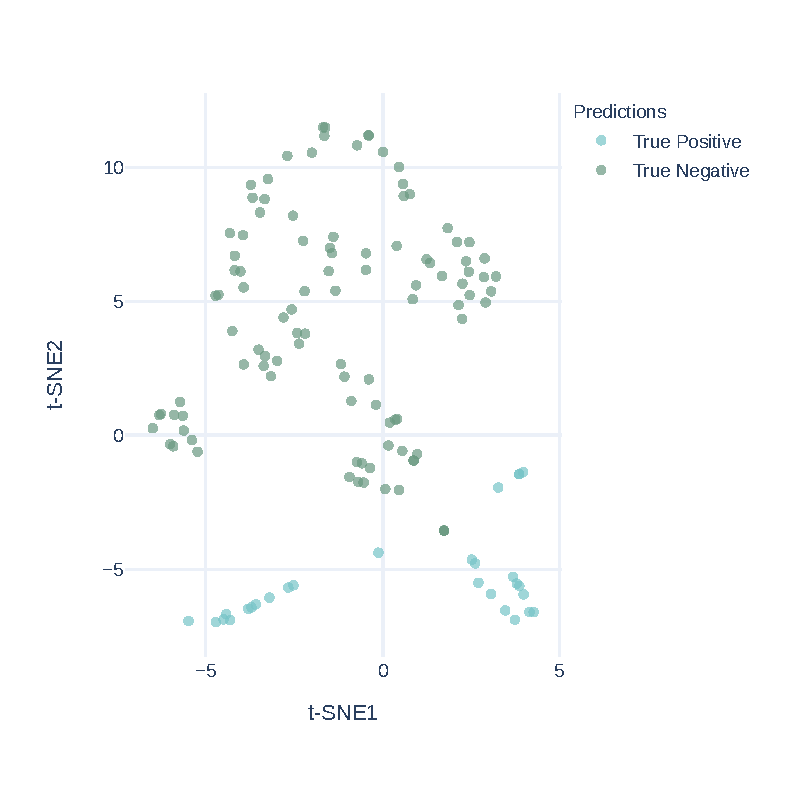
\includegraphics[width=5.52cm]{img/tsne-predictions-pca.pdf}}}%
    \qquad
    \subfloat[\centering Invariants Mining]{{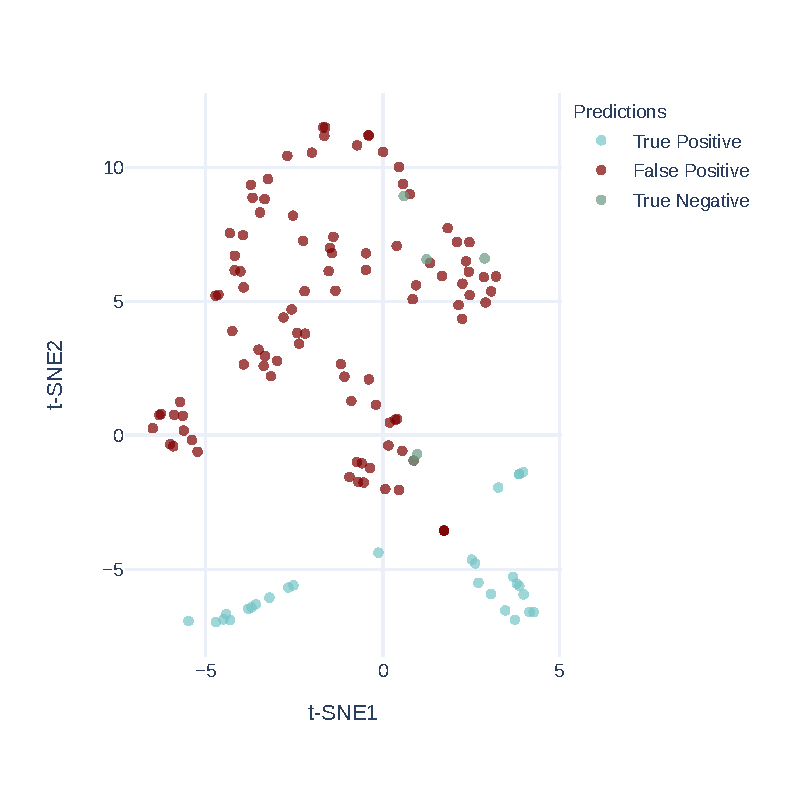
\includegraphics[width=5.52cm]{img/tsne-predictions-invariants-mining.pdf}}}%
    \qquad
    \subfloat[\centering Log Clustering]{{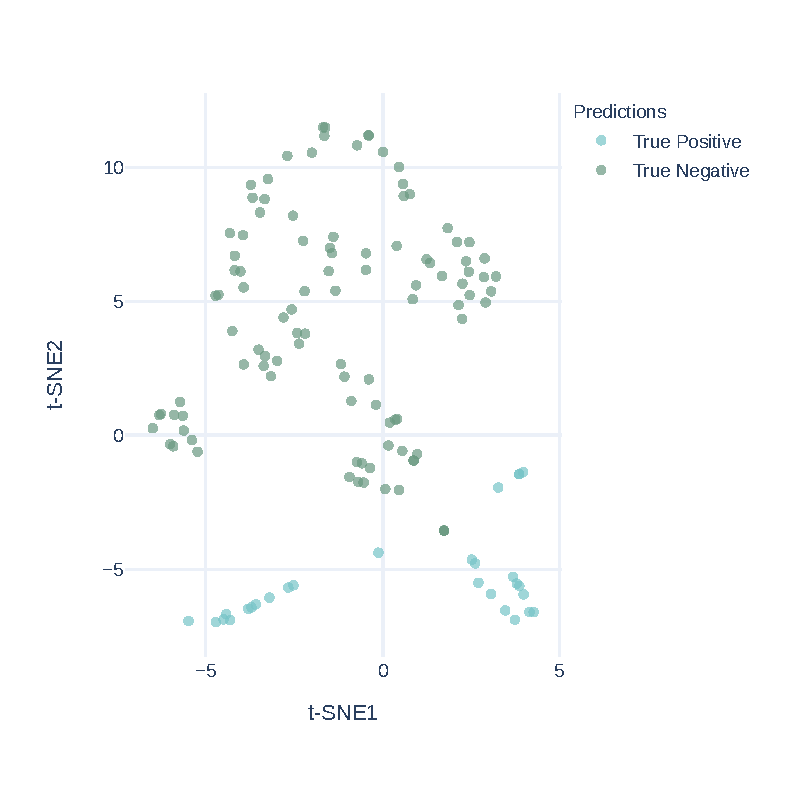
\includegraphics[width=5.52cm]{img/tsne-predictions-clustering.pdf}}}%
    \caption{Comparison of the predictions of Isolation Forest (a), PCA (b), Invariants Mining (c), and Log Clustering (d) on the labeled test data set. It can be observed from the plots that PCA and Log Clustering algorithms handle testing dataset with a $100 \%$ accuracy.}%
    \label{fig:tsne-predictions-labeled}%
\end{figure}


\begin{table}[!h]
\centering
\begin{tabular}{cccc}
\multicolumn{1}{r}{}                 &                              & \textbf{Predicted}          &   $\hat{l}$                          \\ \cline{3-4} 
                                     & \multicolumn{1}{l|}{}        & \multicolumn{1}{l|}{Anomaly} & \multicolumn{1}{l|}{Normal} \\ \cline{2-4} 
                                      
\multicolumn{1}{l|}{\textbf{Actual}} & \multicolumn{1}{l|}{Anomaly}  & \multicolumn{1}{l|}{\textcolor{customBlue}{\textbf{19}}}     & \multicolumn{1}{l|}{\textcolor{customRed}{\textbf{9}}}      \\ \cline{2-4} 
\multicolumn{1}{c|}{\textit{l}}                & \multicolumn{1}{c|}{Normal} & \multicolumn{1}{l|}{\textcolor{customDarkRed}{\textbf{10}}}     & \multicolumn{1}{l|}{\textcolor{customGreen}{\textbf{93}}}      \\ \cline{2-4} 
\end{tabular}
\caption{A confusion matrix for Isolation Forest model on testing dataset.}
\label{table:confusionMatrix:if}
\end{table}


\begin{table}[!h]
\centering
\begin{tabular}{cccc}
\multicolumn{1}{r}{}                 &                              & \textbf{Predicted}          &   $\hat{l}$                          \\ \cline{3-4} 
                                     & \multicolumn{1}{l|}{}        & \multicolumn{1}{l|}{Anomaly} & \multicolumn{1}{l|}{Normal} \\ \cline{2-4} 
                                      
\multicolumn{1}{l|}{\textbf{Actual}} & \multicolumn{1}{l|}{Anomaly}  & \multicolumn{1}{l|}{\textcolor{customBlue}{\textbf{28}}}     & \multicolumn{1}{l|}{\textcolor{customRed}{\textbf{0}}}      \\ \cline{2-4} 
\multicolumn{1}{c|}{\textit{l}}                & \multicolumn{1}{c|}{Normal} & \multicolumn{1}{l|}{\textcolor{customDarkRed}{\textbf{0}}}     & \multicolumn{1}{l|}{\textcolor{customGreen}{\textbf{103}}}      \\ \cline{2-4} 
\end{tabular}
\caption{A confusion matrix for PCA model on testing dataset.}
\label{table:confusionMatrix:pca}
\end{table}


\begin{table}[!h]
\centering
\begin{tabular}{cccc}
\multicolumn{1}{r}{}                 &                              & \textbf{Predicted}          &   $\hat{l}$                          \\ \cline{3-4} 
                                     & \multicolumn{1}{l|}{}        & \multicolumn{1}{l|}{Anomaly} & \multicolumn{1}{l|}{Normal} \\ \cline{2-4} 
                                      
\multicolumn{1}{l|}{\textbf{Actual}} & \multicolumn{1}{l|}{Anomaly}  & \multicolumn{1}{l|}{\textcolor{customBlue}{\textbf{28}}}     & \multicolumn{1}{l|}{\textcolor{customRed}{\textbf{0}}}      \\ \cline{2-4} 
\multicolumn{1}{c|}{\textit{l}}                & \multicolumn{1}{c|}{Normal} & \multicolumn{1}{l|}{\textcolor{customDarkRed}{\textbf{98}}}     & \multicolumn{1}{l|}{\textcolor{customGreen}{\textbf{5}}}      \\ \cline{2-4} 
\end{tabular}
\caption{A confusion matrix for Invariants Mining model on testing dataset.}
\label{table:confusionMatrix:im}
\end{table}

\begin{table}[!h]
\centering
\begin{tabular}{cccc}
\multicolumn{1}{r}{}                 &                              & \textbf{Predicted}          &   $\hat{l}$                          \\ \cline{3-4} 
                                     & \multicolumn{1}{l|}{}        & \multicolumn{1}{l|}{Anomaly} & \multicolumn{1}{l|}{Normal} \\ \cline{2-4} 
                                      
\multicolumn{1}{l|}{\textbf{Actual}} & \multicolumn{1}{l|}{Anomaly}  & \multicolumn{1}{l|}{\textcolor{customBlue}{\textbf{28}}}     & \multicolumn{1}{l|}{\textcolor{customRed}{\textbf{0}}}      \\ \cline{2-4} 
\multicolumn{1}{c|}{\textit{l}}                & \multicolumn{1}{c|}{Normal} & \multicolumn{1}{l|}{\textcolor{customDarkRed}{\textbf{0}}}     & \multicolumn{1}{l|}{\textcolor{customGreen}{\textbf{103}}}      \\ \cline{2-4} 
\end{tabular}
\caption{A confusion matrix for Log Clustering model on testing dataset.}
\label{table:confusionMatrix:clustering}
\end{table}


\section{Expert Validation}

Thanks to the developers of Motorola Solutions, we were able to obtain external validation of our results. We consulted experts to evaluate the detected anomalies, but also to evaluate samples detected as normal by two of the best performing anomaly detection models: PCA and Log Clustering.

Figure \ref{fig:expert-validation-unlabeled-plots} shows the t-SNE plots of the predictions for the Daily data obtained by the trained PCA and Log Clustering models. The Daily dataset is plotted on top of the normal data points for a more convenient visual comparison. For t-SNE and PCA plots produced on the predictions of the Daily dataset by the other less performing algorithms studied in our research, see Appendix \ref{fig:tsne-unlabeled-plots-appendix} and Appendix \ref{fig:pca-unlabeled-plots-appendix}, respectively. 
\begin{figure}
    \centering 
    \subfloat[\centering Log Clustering]{{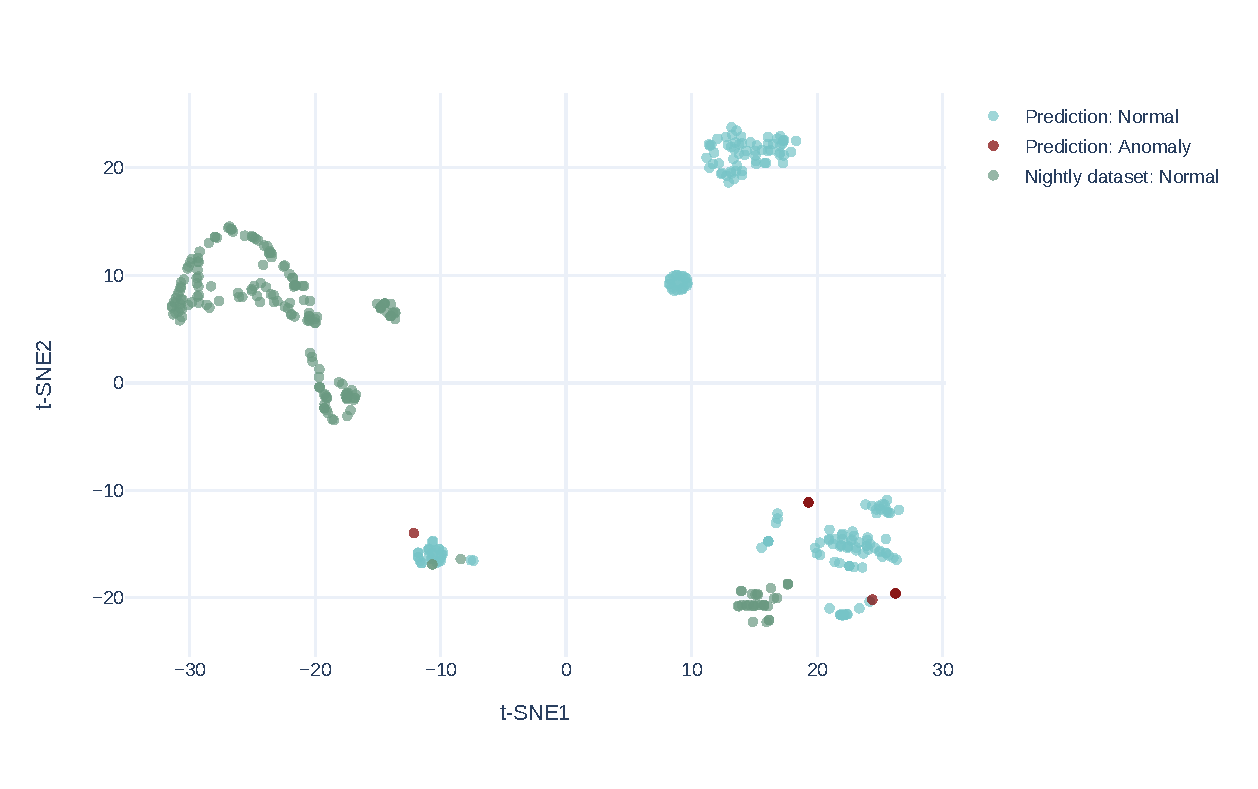
\includegraphics[width=0.9\textwidth]{img/tsne-predictions-unlabeled-clustering.pdf}}} 
    \qquad 
    \subfloat[\centering PCA]{{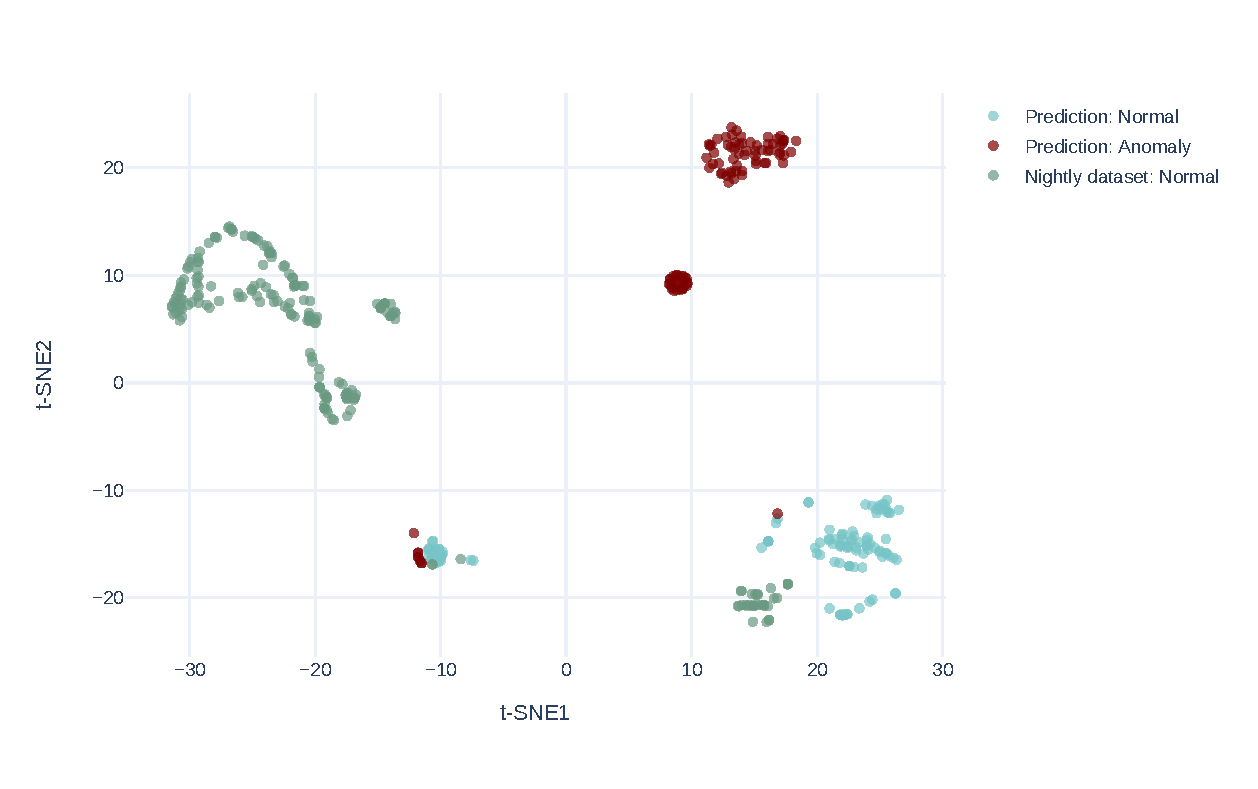
\includegraphics[width=0.9\textwidth]{img/tsne-predictions-unlabeled-pca.pdf}}}
    \caption{Comparison of Log Clustering (a) and PCA (b) predictions on the unlabeled Daily dataset. Green data points represent the normal data points as a reference point, blue and red highlighted data points represent predictions of a normal and anomalous log sequence, respectively.} 
    \label{fig:expert-validation-unlabeled-plots}
\end{figure}

\subsection{Analysis}
The goal of this step was to expose our machine learning models to anomalies that are difficult to simulate manually, or that we are unaware of and thus could not validate against on a larger scale. However, since our models are designed to be able to identify anomalies not seen before, we studied a random sample from the experimental environment during the day. It should follow a very different distribution compared to both the Nightly dataset and the dataset with known anomalies.

The experts were given a small sample of time windows extracted from the Daily dataset. The sample of $12$ windows was given to them in the form of both a \textit{histogram} of event templates and a sequence of \textit{raw logs}. The specific time windows were selected based on their predicted label, so that each predicted class had multiple representative windows in the sample for the two of the best performing anomaly detection models, Log Clustering and PCA. We attempted to select time windows whose predicted labels differed between the models as well as those that were the same.

In these windows, the domain experts managed to identify an anomaly where information from UDP packets is discarded. The packets usually carry the audio information of the calls and their loss can be caused by poor connectivity, which can reduce the overall quality of the calls sent or received. This is certainly a valid anomaly to be detected. 

Upon closer inspection, we noticed that the cluster in the upper right corner corresponds to the anomaly of a discarded packet. As can be seen in Figure~\ref{fig:expert-validation-unlabeled-plots}, this behaviour was only detected as an anomaly by PCA. On the other hand, Log Clustering is less sensitive to the cluster containing calls with larger pocket loss. When this specific anomaly occurs, it does not trigger any other processes in the system and it continues to run as usual trying to deliver them based on best-effort delivery, therefore it can also be argued that a UDP dropout of small size is not an anomaly that needs to raise alarm. The fact that Log Clustering did not recognize these points as anomalies could be fixed by adjusting hyperparameters.

Additionally, the experts did not report any false negatives (anomalies labeled as anomaly free by our models). This information on its own however doesn't prove that there are no instances of those.
Clearly, it is more difficult to identify a false negative by hand. In general, there would be a majority of windows labeled as anomaly-free and we cannot expect human to crawl through all of them effectively verifying that no false negative occurred in the analyzed time span. It is understandable, that a bare eye is not able to spot these just based on the histogram and logs assigned to each of the windows, that are meant for troubleshooting the predictions.